\documentclass{article}
\usepackage{tikz}
\usepackage{pgf}
\usetikzlibrary{datavisualization}
%%%%!!!!!!!!!!!!!!!!!!!!!!
\usetikzlibrary{datavisualization.formats.functions}
\tikzset{help lines/.style=very thin}
\tikzset{Karl’s grid/.style={help lines,color=blue!50}}
%...
%\draw[Karl’s grid] (0,0) grid (5,5);
\begin{document}
\begin{tikzpicture}
	\draw (-1.5, 0) -- (1.5, 0);
	\draw (0, -1.5) -- (0, 1.5);
\end{tikzpicture}
\tikz \draw (-1.5,0) -- (1.5,0) -- (0,-1.5) -- (0,1.5);
\begin{tikzpicture}
	\filldraw [gray] (0, 0) circle (2pt)
						 (1, 1) circle (2pt)
						 (2, 1) circle (2pt)
						 (2, 0) circle (2pt);
	\draw (0, 0) .. controls (1, 1)  and (2, 1) .. (2, 0) 
		   	   		.. controls (4, 1) and (4, -2).. (2, 0);
\end{tikzpicture}
\begin{tikzpicture}
	\draw (-1.5,0) -- (1.5,0);
	\draw (0,-1.5) -- (0,1.5);
	\draw (-1,0) .. controls (-1,0.555)  .. (0,1)
					.. controls (0.555,1) and (1,0.555) .. (1,0);
\end{tikzpicture}
\tikz \draw (0,0) circle (10pt);
\tikz \draw (0,0) ellipse (20pt and 10pt);
\begin{tikzpicture}
\draw (-1.5,0) -- (1.5,0);
\draw (0,-1.5) -- (0,1.5);
\draw (0,0) circle (1cm);
\end{tikzpicture}
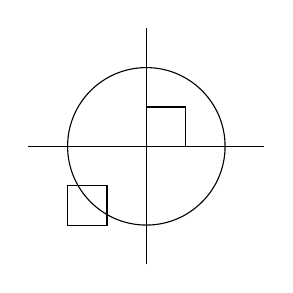
\begin{tikzpicture}
\draw (-1.5,0) -- (1.5,0);
\draw (0,-1.5) -- (0,1.5);
\draw (0,0) circle (1cm);
\draw (0,0) rectangle (0.5,0.5);
\draw (-0.5,-0.5) rectangle (-1,-1);
\end{tikzpicture}
% Grid Path Construction
\tikz \draw[step=.5cm] (-1.4,1.4) grid (1.4,1.4);
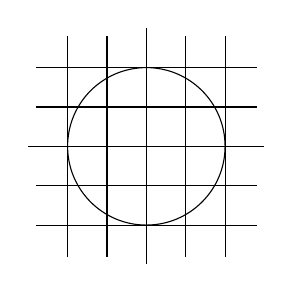
\begin{tikzpicture}
\draw (-1.5,0) -- (1.5,0);
\draw (0,-1.5) -- (0,1.5);
\draw (0,0) circle (1cm);
\draw[step=.5cm] (-1.4,-1.4) grid (1.4,1.4);
\end{tikzpicture}
% 有次序
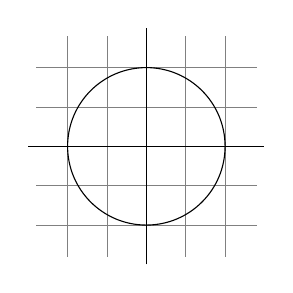
\begin{tikzpicture}
%%%
% ultra thin
% very thin
% thin
% semithick
% thick
% very thick
% ultra thick
%%%
%%%
% loosely dashed
% densely dashed
% loosely dotted
% densely dotted
% dash pattern

\draw[step=.5cm,gray,very thin] (-1.4,-1.4) grid (1.4,1.4);
\draw (-1.5,0) -- (1.5,0);
\draw (0,-1.5) -- (0,1.5);
\draw (0,0) circle (1cm);
\end{tikzpicture}
\begin{tikzpicture}
[Karl’s grid/.style ={help lines,color=#1!50},
Karl’s grid/.default=blue]
\draw[Karl’s grid] (0,0) grid (1.5,2);
\draw[Karl’s grid=red] (2,0) grid (3.5,2);
\end{tikzpicture}
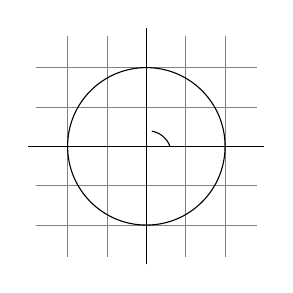
\begin{tikzpicture}
\draw[step=.5cm,gray,very thin] (-1.4,-1.4) grid (1.4,1.4);
\draw (-1.5,0) -- (1.5,0);
\draw (0,-1.5) -- (0,1.5);
\draw (0,0) circle (1cm);
\draw (3mm,0mm) arc (20:80:3mm);
\end{tikzpicture}
\begin{tikzpicture}[scale=3]
\draw[step=.5cm,gray,very thin] (-1.4,-1.4) grid (1.4,1.4);
\draw (-1.5,0) -- (1.5,0);
\draw (0,-1.5) -- (0,1.5);
\draw (0,0) circle (1cm);
\draw (4mm,2mm) arc (0:30:3mm);
\end{tikzpicture}
\tikz \draw (0,0) arc (0:315:1.75cm and 1cm);
%% Clipping a Path
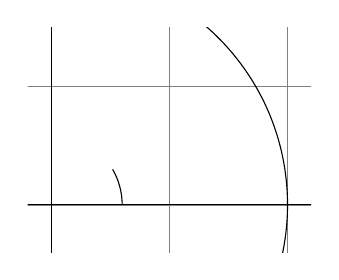
\begin{tikzpicture}[scale=3]
\clip (-0.1,-0.2) rectangle (1.1,0.75);
\draw[step=.5cm,gray,very thin] (-1.4,-1.4) grid (1.4,1.4);
\draw (-1.5,0) -- (1.5,0);
\draw (0,-1.5) -- (0,1.5);
\draw (0,0) circle (1cm);
\draw (3mm,0mm) arc (0:30:3mm);
\end{tikzpicture}
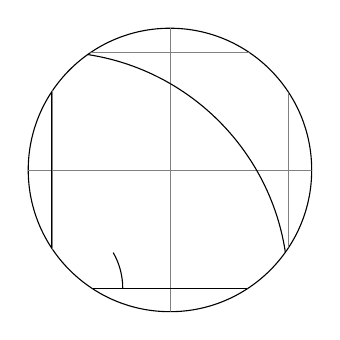
\begin{tikzpicture}[scale=3]
\clip[draw] (0.5,0.5) circle (.6cm);
\draw[step=.5cm,gray,very thin] (-1.4,-1.4) grid (1.4,1.4);
\draw (-1.5,0) -- (1.5,0);
\draw (0,-1.5) -- (0,1.5);
\draw (0,0) circle (1cm);
\draw (3mm,0mm) arc (0:30:3mm);
\end{tikzpicture}
\tikz \draw (0,0) rectangle (1,1) (0,0) parabola (1,1);
\tikz \draw[x=1pt,y=1pt] (0,0) parabola bend (4,16) (6,12);

A sine \tikz \draw[x=1ex,y=1ex] (0,0) sin (1.57,1); curve.
\tikz \draw[x=1.57ex,y=1ex] (0,0) sin (1,1) cos (2,0) sin (3,-1) cos (4,0)
(0,1) cos (1,0) sin (2,-1) cos (3,0) sin (4,1);
%% filling and drawing
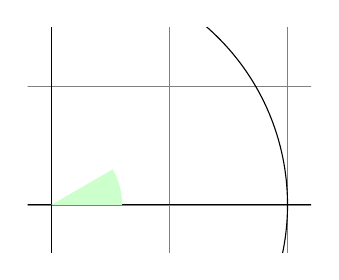
\begin{tikzpicture}[scale=3]
\clip (-0.1,-0.2) rectangle (1.1,0.75);
\draw[step=.5cm,gray,very thin] (-1.4,-1.4) grid (1.4,1.4);
\draw (-1.5,0) -- (1.5,0);
\draw (0,-1.5) -- (0,1.5);
\draw (0,0) circle (1cm);
\fill[green!20!white] (0,0) -- (3mm,0mm) arc (0:30:3mm) -- (0,0);
\end{tikzpicture}
%\fill[green!20!white] (0,0) -- (3mm,0mm) arc (0:30:3mm) -- cycle;
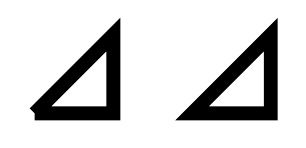
\begin{tikzpicture}[line width=5pt]
\draw (0,0) -- (1,0) -- (1,1) -- (0,0);
\draw (2,0) -- (3,0) -- (3,1) -- cycle;
%\useasboundingbox (0,1.5); % make bounding box higher
\end{tikzpicture}
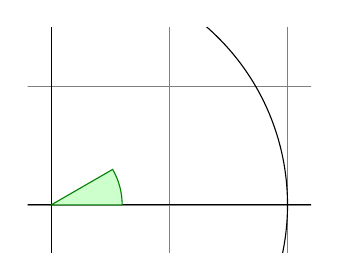
\begin{tikzpicture}[scale=3]
\clip (-0.1,-0.2) rectangle (1.1,0.75);
\draw[step=.5cm,gray,very thin] (-1.4,-1.4) grid (1.4,1.4);
\draw (-1.5,0) -- (1.5,0);
\draw (0,-1.5) -- (0,1.5);
\draw (0,0) circle (1cm);
\filldraw[fill=green!20!white, draw=green!50!black]
(0,0) -- (3mm,0mm) arc (0:30:3mm) -- cycle;
\end{tikzpicture}
%% shade
\tikz \shade (0,0) rectangle (2,1) (3,0.5) circle (.5cm);
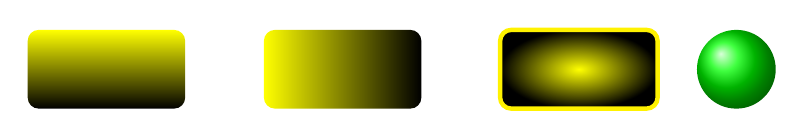
\begin{tikzpicture}[rounded corners,ultra thick]
\shade[top color=yellow,bottom color=black] (0,0) rectangle +(2,1);
\shade[left color=yellow,right color=black] (3,0) rectangle +(2,1);
\shadedraw[inner color=yellow,outer color=black,draw=yellow] (6,0) rectangle +(2,1);
\shade[ball color=green] (9,.5) circle (.5cm);
\end{tikzpicture}
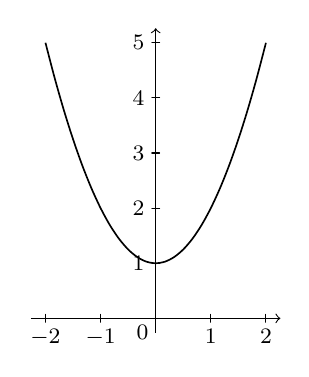
\begin{tikzpicture}[scale=.7]
\datavisualization [school book axes, visualize as smooth line]
data [format=function] {
var x : interval [-2:2];
func y = \value x*\value x + 1;
};
\end{tikzpicture}


\end{document}